\section{Mise en place des maquettes}

	Dans cette partie, nous allons détailler les trois architectures mise en place pour la création d'un VPN.Nous commenceront par détailler la solution VPN que Microsoft propose.

\subsection{Solution Windows}
	Pour ce projet, nous avons décider d'installer Windows Server 2003 Entreprise Edition, afin d'avoir un sytème d'exploitation récent. Toutes les fonctionnalités utilisées pour la création d'un VPN sont incluses dans cette version. Il n'y a pas besoin d'installer une application tierce.
	Voyons à présent les différents services nécessaires pour la mise en place du VPN de Microsoft.

\subsubsection{Côté serveur : les services installés}

	Afin de pouvoir se mettre dans les conditions du réseau interne de l'ISIMA, nous avons décidé de configurer plusieurs services:
~


\begin{itemize}
	\item  DHCP,
	\item  DNS, 
	\item  Active Directory,
	\item  Routage et accès distant (VPN),
	\item  Autorité de certification (CA).
\end{itemize}
~
Il est à noter que pour pouvoir installer l'autorité de certification, il faut dans un premier temps installer le service IIS.	

	Ces nombreux services sont nécessaires pour la création d'un VPN. A présent, détaillons la configuration de chacun de ces servives. 
	Remarque : Sous windows on ne parle pas de serveur mais de service. Tout les fonctionnalités de la machine (DNS, DHCP ou autre) sont référencés comme des services.


\paragraph{Caractéristique de la machine}
~\

Le serveur windows est installé sur un DELL PowerEdge 1300. Il est doté d'un processeur INTEL de type Pentium II cadencé à 348 Mhz. Il possède 512 Mo de mémoire vive et un disque dur de 9 Go.
Le serveur est composé de trois cartes réseaux, une pour le réseau extérieur et deux autres pour le réseau interne. 



Voici leur adresse IP:

\begin{figure}[H]
	\begin{center}
\begin{tabular}{|l|c|c|}
\hline
Caractéristique & Réseau & Adresse IP \\
\hline
Realtek RTL 8139 Familly & réseau PROFS & 10.0.0.11/24 \\
Realtek RTL 8139 Familly & réseau extérieur & 192.168.102.250/24 \\
Fast Ethernet CNET PRO 200P & réseau STUDENTS & 192.168.0.11/24 \\
\hline
\end{tabular}
	\end{center}
	\caption{Caractéristique des cartes réseaux}
	\label{IP_carte_reseau}
\end{figure}

Tout les cartes installés sont de type 100Mbit/s.
~

\paragraph{Service DHCP}
~\


Ce service est nécessaire pour l'attribution des adresses IP qui seront allouées aux différents clients lors de leurs connexion au serveur VPN. Nous avons configurer le service DHCP de la manière suivante. Sachant que le serveur VPN doit avoir deux cartes réseaux indépendantes (une sur le réseau STUDENTS et une sur le réseau PROFS) le DHCP peut fournir deux pools d'adresse différents. 
Voici les caractéristiques des deux réseaux:

\begin{figure}[H]
	\begin{center}
\begin{tabular}{|l|c|c|}
\hline
Caractéristique & Réseau PROFS & Réseau STUDENTS \\
\hline
Désignation Carte réseau & DHCP\_PROFS & DHCP\_STUDENTS \\
Adresse IP Carte réseau & 10.0.0.11 & 192.168.0.11 \\
Pool d'adresse & 10.0.2.100 à 10.0.2.254 & 192.168.0.100 à 192.168.0.254 \\
Masque réseau & 255.255.255.0 & 255.255.255.0 \\
Serveur DNS/routeur & 10.0.0.11 & 192.168.0.11 \\
Nom du domaine DNS & wvpn.isima.fr & wvpn.isima.fr \\
\hline
\end{tabular}
	\end{center}
	\caption{Caractéristique du service DHCP}
	\label{service_DHCP}
\end{figure}

Il est à noter que lors de l'installation du service DHCP, et en dehors des différentes configurations des cartes, il n'y a pas d'options spécifiques. Ce sont les options par défaut.
Il est à remarquer que le service DHCP se compose de deux étendues, une pour chaque carte. Cependant, le service DHCP s'attache à une seule carte réseau et non au deux. Dans la maquette, le service se lie avec la carte DHCP\_PROFS. Pour illustrer ces propos, voici un screenshot du service DHCP.

\begin{figure}[H]
	\begin{center}
	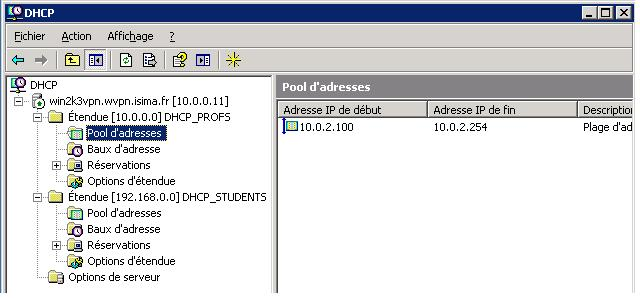
\includegraphics[width=\textwidth]{partie_2/screen_windows/dhcp.JPG}\\
	\end{center}
	\caption{Lien avec la carte réseau DHCP\_PROFS}
	\label{Screen_client_dhcp}
\end{figure}


On remarque que bien que la présence des deux étendues et que la carte DHCP\_PROFS (10.0.0.11) s'attache au service DHCP.
~\


Voyons à présent la configuration du service DNS.

\paragraph{Service DNS}
~\


Afin de pouvoir utiliser l'active directory nous avons du installer ce service. Celui-ci nous permet de résoudre les différentes adresses IP qui seront nécessaire lorsq'un client VPN se connectera sur le réseau interne.
Voici les caractèristiques du service DNS:
~\


\begin{figure}[H]
	\begin{center}
\begin{tabular}{|l|c|c|}
\hline
Caractéristique & Serveur Windows2003 \\
\hline
Nom de la machine &  win2k3vpn\\
Nom du domaine & wvpn.isima.fr\\
Type de zone &  zone principale\\
\hline
\end{tabular}
	\end{center}
	\caption{Caractéristique du service DNS}
	\label{service_DNS}
\end{figure}

~\

Il est à remarquer que lors de l'installation du service, nous avons décider d'incorporer la zone de recherche inversée. Le serveur windows étant composé de trois cartes réseaux, il y a trois zones. Afin de vérifier que le service DNS est bien configurer, la commande NSLOOKUP nous permet de tester le DNS. 
L'illustration suivante montre la résolution DNS est correcte.

\begin{figure}[H]
	\begin{center}
		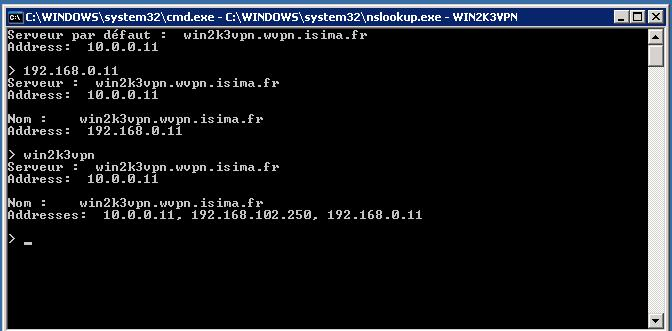
\includegraphics[width=\textwidth]{partie_2/screen_windows/nslookup.JPG}\\
	\end{center}
	\caption{Résolution DNS}
	\label{NSLOOKUP}
\end{figure}

Tout comme le service DHCP, le service DNS se lie avec une seule carte réseau. 

Intéressons nous à présent à la configuration de l'Active Directory.

\paragraph{Active Directory}
~\

Ce service nous a permi de créer un annuaire afin d'indentifier les clients souhaitant se connecter sur le réseau interne. Afin de pouvoir effectuer des tests sur la connexion VPN, nous avons dans un premier temps créeer deux groupes: un groupe STUDENTS et un groupe PROFS.

Il est à noter que lorsqu'on crée un utilisateur, on doit l'ajouter dans le groupe PROFS ou STUDENTS sans oublier de lui donner l'autorisation de pouvoir se connecter. 

\begin{figure}[H]
	\begin{center}
		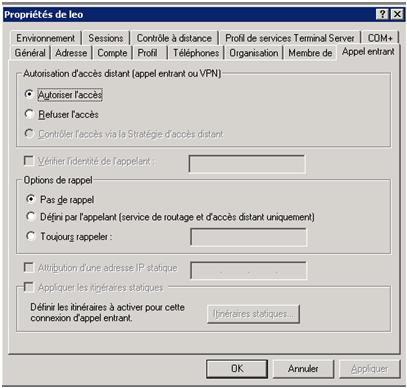
\includegraphics[width=0.50\textwidth]{partie_2/screen_windows/vpn.JPG}\\
	\end{center}
	\caption{Autorisation de se connecter via VPN sur le serveur Windows 2k3}
	\label{VPN_AUTORISATION}
\end{figure}

Du point de vue de la stratégie de groupe (GPO) nous avons décider de laisser la configuration par défaut.

Une fois les services de base installé, voyons à présent la configuration du service de \textit{Routage et accès distant} .

\paragraph{Routage et accès distant}
~\


Le service routage et accès distant est le service qui va nous permettre de monter un tunnel sécurisé. Lors de l'installation du service, l'administrateur doit choisir l'option ``routage pour réseaux locaux uniquement'' ainsi que l'option ``serveur d'accès distant''. Une fois le service installé, il faut configurer les options de sécurité qui sont propre au serveur (un clique droit sur le nom du serveur permet de modififer les propriétés). Cela correspond à la manière que les utilisateurs s'identifie. Le service propose deux choix : identification par l'annuaire ou bien en utilisant un serveur RADIUS.

\begin{figure}[H]
	\begin{center}
		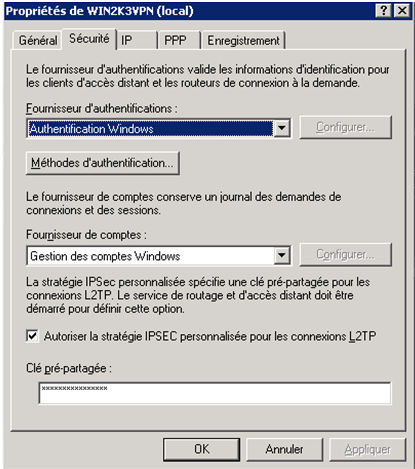
\includegraphics[width=0.50\textwidth]{partie_2/screen_windows/secu_vpn.PNG}\\
	\end{center}
	\caption{Choix de la méthode d'authentification}
	\label{VPN_AUTHENTIFICATION}
\end{figure}

Nous avons essayer de tester la maquette en utilisant le serveur RADIUS afin que celui-ci authentifie l'utilisateur avec la base NIS. Cependant les essais n'ont pas été concluant, nous n'avons pas pu nous identifier en utilisant notre compte ISIMA. Afin de rendre la maquette fonctionnel, nous avons dû laisser l'authentification par l'intermédiaire de l'annuaire local.

Dans l'onglet IP, il faut configurer la manière dont le service va distribuer les adresses IP. Ici nous avons le choix, soit le système gère les adresses IP en utilisant le service DHCP, soit l'administrateur peut remplir manuellement la plage d'adresse IP. La dernière option ``carte'' qui correpond à un menu déroulant nous permettant de selectionner la carte réseau qui repondrera aux demandes de la création d'un tunnel sécurisé. 

\begin{figure}[H]
	\begin{center}
		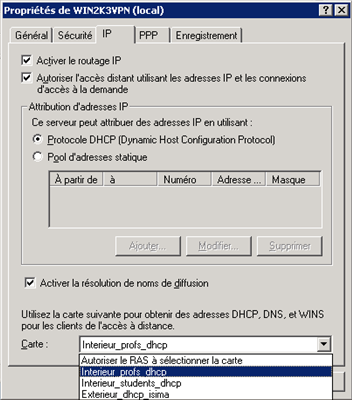
\includegraphics[width=0.50\textwidth]{partie_2/screen_windows/choix_carte.PNG}\\
	\end{center}
	\caption{Selection de l'interface réseau}
	\label{VPN_CARTE_ECOUTE}
\end{figure}

En naviguant dans les différentes options, on se rend rapidement compte que le service d'accès distant se lie avec une seule carte réseau. C'est la grande limitation. Il n'est pas possible que les deux cartes réseaux destinés pour le traffic interne redirige les différents flux réseaux.

D'un point de vue sécurité, il est possible de créer des stratégies d'accès distant. Pour le projet, nous avons créer une stratégie avec les spécifications suivantes:
~\
\begin{itemize}
 	\item Appartenance à un groupe : PROFS ou STUDENTS
	\item Type d'authentification : MS-CHAP V2
	\item Spécification du type de connexion : VPN
\end{itemize}
~


Cette stratégie d'accès distant comporte une priorité de 1. Si un client respecte tous ces critères il pourra alors se connecter sur le serveur VPN.

\begin{figure}[H]
	\begin{center}
		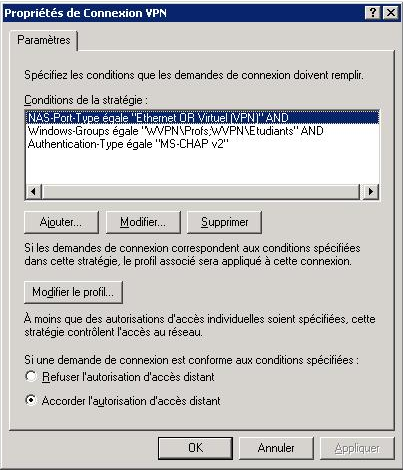
\includegraphics[width=0.50\textwidth]{partie_2/screen_windows/strat.png}\\
	\end{center}
	\caption{Stratégie d'accès distant}
	\label{VPN_STRAT}
\end{figure}

Dans la stratégie d'accès on peut rajouter un paramètre sur la date. En effet, on le paramétrant, on peut définir une plage horaire où l'utilisateur ne pourra pas se connecter.

Concernant le tyoe d'authentification, on utilise le protocole MS-CHAP V2 qui est un protocole propriétaire de Miscrosoft. En complement de cela, le serveur VPN fait un challenge de type MD5 afin d'authentifier le client.

Le protocole MS-CHAP V2 utilise une authentification mutuelle. Cela permet au serveur d'authentification et à la machine distante de vérifier leurs identités respectives. L'inconvenient de cette méthode est que le login du client passe en clair sur le réseau. En sniffant la connexion par l'intermédiare de Wireshark, nous nous sommes rendu compte de cela. Par contre, le challenge MD5, et les mots de passe sont chiffrés.



Afin d'améliorer la sécurité, nous avons décider de mettre en place une autorité de certification.

\paragraph{Autorité de certification}
~


Cette autorité va nous permettre de délivrer des certificats qui nous seront utile par la suite dans la configuration du routeur CISCO. Pour la configuration de l'autorité nous avons choisi une autorité racine autonome ayant comme nom commun ISIMA. Les certificats ont une validité d'un an. D'un point de vue sécurité, l'autorité utilise l'algorithme de hashage SHA-1 et pour le cryptage on utilise Microsoft Strong Cryptographic Provider. La clé publique est chiffrée grâce à l'algorithme RSA sur 2048 bits.
Pour récupérer un certificat, le client doit se connecter sur l'URL suivante : \verb|http://192.168.102.250/certsrv|
Lorsqu'il se connecte sur cette page, il doit faire une demande de certificat. L'utilisateur a le choix entre un certificat de type WEB ou de type MESSAGERIE. Une fois le choix fait, l'autorité de certification recoit une demande de certificat. L'administrateur doit autoriser ou refuser cette demande. Dans le cas où la demande est validée, l'utilisateur doit se reconnecter à nouveau sur le site WEB afin de pouvoir installer ce certificat sur sa machine.

Cependant, après avoir fait plusieurs essais, la connexion sur le serveur VPN Windows ne se produit pas. Nous pensons que le problème se situe dans la définition de la requête du certificat. Pour l'architecture du VPN Windows, ne nous utiliserons pas d'autorité de certification afin d'augmenter le niveau de sécurité. 

Voyons à présent, la configuration du côté client

\subsubsection{Configuration du client}
~

L'un des avantages majeurs de la solution Windows est que le client VPN est déjà intégrer dans le système d'exploitation de Microsoft. Voici les différentes étapes pour la création d'une connexion VPN.

La 1ère étape consiste à configurer une nouvelle connexion. La connexion de type entreprise permet à l'utilisateur de se connecter au réseau privé. (VPN).

\begin{figure}[H]
	\begin{minipage}{0.5\textwidth}
		\begin{flushleft} \large
			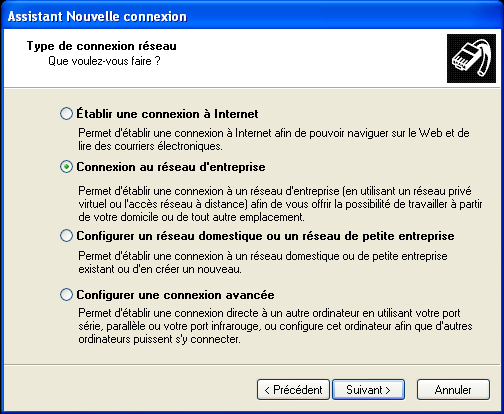
\includegraphics[width=0.95\textwidth]{partie_2/screen_windows/etape1.PNG}\\
		\end{flushleft}
	\end{minipage}
	\begin{minipage}{0.5\textwidth}
		\begin{flushright} \large
			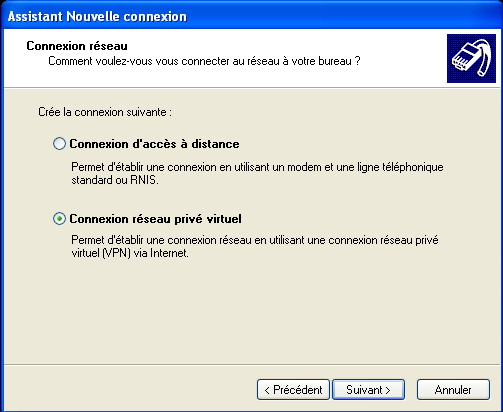
\includegraphics[width=0.95\textwidth]{partie_2/screen_windows/etape2.PNG}\\
		\end{flushright}
	\end{minipage}
	\caption{Configuration d'une nouvelle connexion}
	\label{VPN_ETAPE1}
\end{figure}
~\

La 2ème étape consiste à donner un nom à sa connexion VPN et spécifier si l'on souhaite effectuer une connexion initiale avant la connexion VPN.

\begin{figure}[H]
	\begin{minipage}{0.5\textwidth}
		\begin{flushleft} \large
			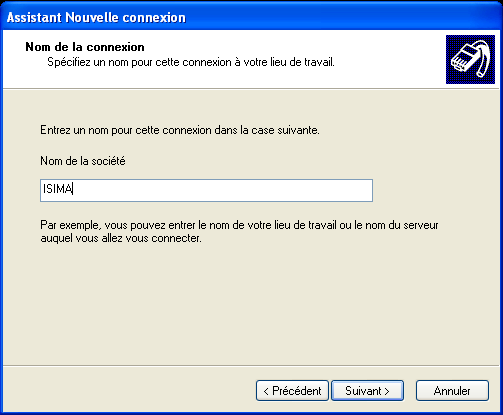
\includegraphics[width=0.95\textwidth]{partie_2/screen_windows/etape3.PNG}\\
		\end{flushleft}
	\end{minipage}
	\begin{minipage}{0.5\textwidth}
		\begin{flushright} \large
			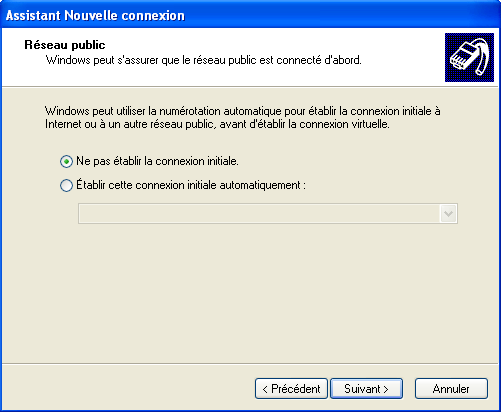
\includegraphics[width=0.95\textwidth]{partie_2/screen_windows/etape4.PNG}\\
		\end{flushright}
	\end{minipage}
	\caption{Configuration nom connexion}
	\label{VPN_ETAPE2}
\end{figure}
~\


La dernière étape est importante car on spécifie l'adresse du serveur qui nous permettera de monter une liaison sécurié. L'utilisateur pourra pour augmenter la sécurité utiliser une carte à puce pour s'authentifier.

\begin{figure}[H]
	\begin{minipage}{0.5\textwidth}
		\begin{flushleft} \large
			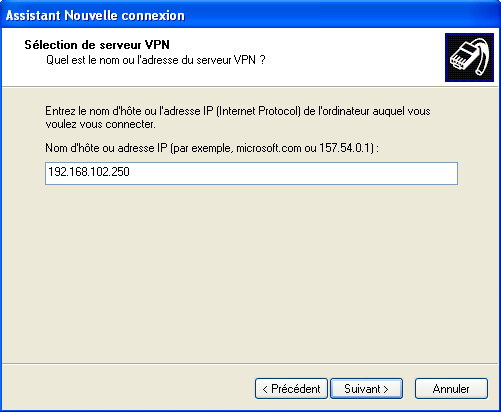
\includegraphics[width=0.95\textwidth]{partie_2/screen_windows/etape5.PNG}\\
		\end{flushleft}
	\end{minipage}
	\begin{minipage}{0.5\textwidth}
		\begin{flushright} \large
			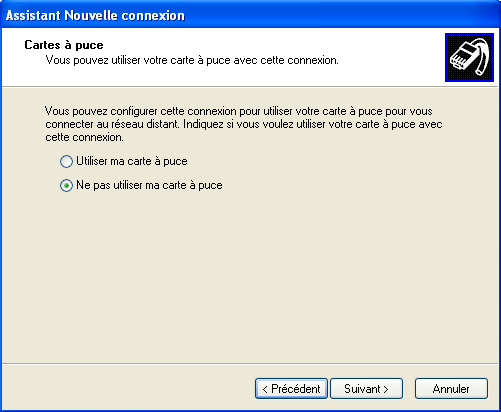
\includegraphics[width=0.95\textwidth]{partie_2/screen_windows/etape6.PNG}\\
		\end{flushright}
	\end{minipage}
	\caption{Configuration adresse IP du serveur VPN}
	\label{VPN_ETAPE3}
\end{figure}

~\

Une fois la nouvelle connexion VPN crée le client va pouvoir désormais se connecter sur le serveur VPN en utilisant un login et un mot de passe qui ont été défini dans l'Active Directory. Nous avons laissé les configurations de sécurité par défaut pour le client.

Pour notre exemple, nous utiliserons l'utilisateur \verb leo. Une fois la connexion accepté par le serveur, voici ce que l'utilisateur peut voir sur son sytème d'exploitation.

\begin{figure}[H]
	\begin{center}
		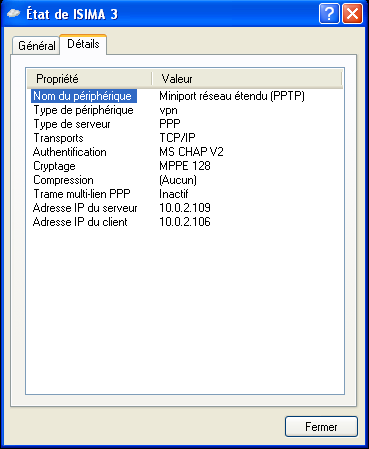
\includegraphics[width=0.50\textwidth]{partie_2/screen_windows/etape7.PNG}\\
	\end{center}
	\caption{Information VPN}
	\label{VPN_ETAPE7}
\end{figure}

~\

Cette image nous montre des informations importantes sur la nature du VPN. Tout d'abord, elle nous informe le protocole qu'elle utilise. Ici on utilise PPTP. Ensuite, le client nous donne le type de connexion : VPN ainsi que sa nouvelle adresse IP : 10.0.2.106
Du point de vue sécurité, l'authentification se fait par l'intermédiaire de MS-CHAP V2 et le chiffrement par le protocole MPPE.

MPPE est le protocole de chiffrement de Microsoft. Il se base l'algorithme RSA RC4. MPPE supporte trois tailles de clés : 40 bits, 56 bits et 128 bits.

Il est à remarquer que sous Windows 2000 la taille de la clé ne dépasse pas les 40 bits. Il ne faut pas oublier d'activer sur le serveur VPN les différents tailles des clés sans quoi la connexion est refusée. 

\begin{figure}[H]
	\begin{center}
		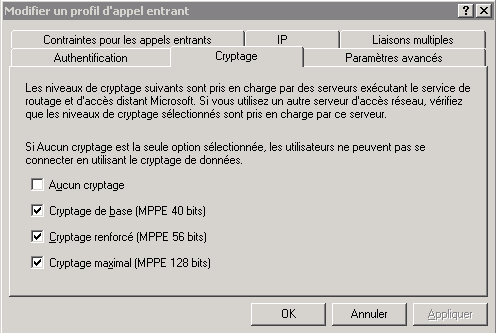
\includegraphics[width=0.50\textwidth]{partie_2/screen_windows/cryptage.PNG}\\
	\end{center}
	\caption{Cryptage MPPE}
	\label{VPN_CRYPTAGE}
\end{figure}


\subsubsection{Bilan et limites de la solution}
~

Microsoft propose une solution VPN très intéressante et facile à mettre en place (côté serveur comme côte client). Cependant, elle est vraiment destiné à des petites structures réseaux. Dans le cas de l'ISIMA, la structure du réseau est plus complexe. En effet, le réseau se compose d'une branche PROFESSEUR et d'une branche ETUDIANT. L'inconvenient majeur de Microsoft est que chaque service doit se lier avec une seule carte réseau. Il est donc impossible de dissocier le trafic réseau sur les deux cartes, ce qui ne respecte pas le cachier des charges du projet. La solution serait de virtualiser un serveur Windows 2003 et de lier la carte réseau virtuel à la carte réseau physique de la machine. Sous VMware par exemple, il faudrait utiliser le mode bridgé pour les cartes réseaux.

Du point de vue client, nous n'avons pas réussi à nous connecter avec une plateforme LINUX à cause d'une mauvaise implementation du protocole PPTP.


Concernant la récupération des login et des mots de passe de l'ISIMA, nous avons décider de ne pas interfacer notre maquette, car le service VPN se lie avec une seule carte réseau. Ceci nous empeche de gérer le réseau et de savoir quelle type d'utilisateur est connecté (PROF ou ELEVE). Cependant, la procédure à suivre serait de rajouter sur le domaine de l'ISIMA le serveur Windows et de lancer une réplication de la base Active Directory. 
Si l'on souhaite utiliser la base NIS de l'ISIMA Microsoft propose une suite d'outil \verb| Windows Service for UNIX| téléchargeable directement sur le site. Cette suite propose d'intégrer à Windows les commandes d'UNIX. On pourra par exemple utiliser les commandes YPCAT. Une des améliorations possible de la maquette serait de récuperer toutes les informations des personnes de l'ISIMA via ces outils. L'interopérabilité serait complète.

D'un point de vue sécurité, sans l'utilisation de certificats, le mot de passe du client est crypté. Par contre le login du client et le nom de la machine est en clair sur le réseau pendant la phase du challenge MD5. 
Voici une trace issue de Wireshark qui montre ce problème de sécurité.

\begin{figure}[H]
	\begin{center}
		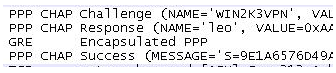
\includegraphics[width=0.5\textwidth]{partie_2/screen_windows/connexion.png}\\
	\end{center}
	\caption{Trace d'une connexion}
	\label{VPN_CONNEXION}
\end{figure}


Par rapport à l'autorité de certifications, nous avons été capable de générer des certificats et les installer sur les machines tests. Par contre, la connexion avec le serveur VPN n'a pas pu s'établir. A l'heure actuel nous ne savons toujours pas d'où provient le problème. Nous soupçonnons un problème de communication entre l'autorité de certification et la machine test.

Après avoir expliquer la configuration du serveur Windows 2003 et ses limitations, intéressons nous à la solution VPN sous Linux avec le logiciel OpenVPN.
 




\subsubsection{Solution dans son fonctionnement}
\subsubsection{Limites de la solution}
% 
% \subsection{Solution Linux}
% \subsubsection{Configuration du VPN}
% \subsubsection{Sécurité+protocoles}
% \subsubsection{Limites de la solution}

\section{OpenVPN}

\subsection{Introduction}

\subsubsection{Généralités}
OpenVPN est un outil Open-Source permettant de créer des tunnels sécurisés (SSL/TLS) à travers un réseau non sûr comme Internet. OpenVPN est à la fois facile à installer et à configurer, en plus d'être disponible sur à peut prêt toutes les plates-formes (Linux, Windows, BSD, Mac OS, Solaris). Le principe de configuration reste le même quelque soit la plate-forme utilisée.

OpenVPN est basé sur une architecture client-server. Le VPN fonctionne soit site-à-site, soit avec des clefs partagées. Les données sont tunnelisées sur un seul port, TCP ou UDP.

\subsubsection{Les deux types de VPN}
Il existe deux types de VPN : les VPN bridgés et les VPN routés. Dans le cas du mode bridgé le réseau virtuel créé devient une réelle extension du réseau local. L'avantage de ce mode est la facilité d'intégration de la solution VPN au sein de l'infrastructure déjà en place. Ce mode est d'ailleurs la seule option si pour une raison ou pour une autre des paquets broadcasts doivent traverser le VPN. Le principal inconvénient de ce mode apparait lors du passage à l'échelle : comme c'est le réseau local qui doit absorber les clients du VPN, il faut suffisament de ressources disponibles (adresses IP, etc.).

Le mode routé est le mode le plus utilisé. Bien que sa mise en place soit plus complexe, ce mode permet de faire du réseau virtuel un réseau à part du réseau local. On est ainsi capable de mettre en place une politique d'accès différente pour les utilisateurs connectés depuis l'extérieur, ce qui renforce encore la sécurité de l'infrastructure. Le second grand aventage des VPN routés est que le passage a l'échelle s'effectue ne pose aucun problème étant donné que l'on n'impacte pas l'utilisation du réseau local.

~

La figure \ref{tableau_types_vpn} résume les avantages et inconvénient de chacun des deux types de VPN :
\begin{figure}[H]
	\begin{center}
		\begin{tabular}{c|c}
			VPN bridgé & VPN routé \\
			\hline
			extension du réseau local & réseau à part \\
			mauvais passage à l'échelle & passage à l'échelle \\
			laisse passer les broadcasts & broadcasts impossibles \\
		\end{tabular}
	\end{center}
	\caption{Avantages et inconvénients des deux types de VPN}
	\label{tableau_types_vpn}
\end{figure}

Nous avons choisi de mettre en place une configuration de VPN routé, car mieux adaptée à l'utilisation que l'ISIMA pourrait en faire.

\subsection{Mise en place côté serveur}

La mise en place de l'infrastructure s'effectue en plusieures étapes. Tout d'abord nous installerons et configurerons OpenVPN sur le serveur, ensuite nous génèrerons les clefs et certificats de sécurité nécessaires, et enfin nous mettrons en place les outils nécessaires pour authentifier les utilisateurs via l'annuaire NIS de l'ISIMA.

\subsubsection{Installation et configuration d'OpenVPN}

La machine fonctionne sous \texttt{Linux CentOS 5.1}. OpenVPN n'étant pas disponible directement dans les paquets de cette distribution, nous allons construire notre propre rpm. Les paquets requis pour mener à bien cette étape sont à installer grâce à la commande suivante :

\verb|[root@centosvpn ~]# yum install openssl-devel pam-devel rpm-build gcc-c++|

~

La version d'OpenVPN utilisée pour le projet est la 2.0.9 disponible sur \verb|http://openvpn.net/|. Celle-ci dépend des paquets \verb|lzo-devel-1.08-fr2.i386| et \verb|lzo-1.08-fr2.i386|, disponibles par exemple sur \verb|http://rpmfind.net/|.

\verb|[root@centosvpn ~]# wget ftp://rpmfind.net/linux/freshrpms/redhat/9/lzo/lzo-devel-1.08-fr2.i386.rpm|

\subsubsection{Génération des clefs et certificats de sécurité}

\subsubsection{Authentification via l'annuaire de l'ISIMA}

OpenVPN étant capable de réaliser une authentification PAM (méthode standart sur les systèmes UNIX), c'est la solution que nous avons retenue. Nous allons donc configurer un client NIS sur la machine de test, et indiquer à OpenVPN comment l'utiliser.

La première étape consiste à installer l'annuaire NIS si ce n'est pas déjà fait (paquet \texttt|ypserv|) à faire entrer la machine dans le domaine NIS de l'ISIMA : .




\pagebreak


% \begin{figure}[H]
% 	\begin{center}
% 		\begin{minipage}{0.90\textwidth}
% 			\begin{lstlisting}[frame=trBL]
% 
% 			\end{lstlisting}
% 		\end{minipage}
% 	\end{center}
% 	\caption{Récupération des éléments de réponse dans un message de commande}
% 	\label{format_reponse_commande}
% \end{figure}


% \subsection{Solution Cisco}
% \subsubsection{Protocoles utilisés}
% \subsubsection{Système d'authentification}
% \subsubsection{Configuration du routeur}
% \subsubsection{Limites de la solution}

\subsection{Solution Cisco}

\subsubsection{Généralités}
ipsec esp-sha1

\subsubsection{Mise en place côté serveur}


\paragraph{Configuration de base}
~

Commençons par configurer les interfaces du routeur. L'interface connectée au réseau de l'ISIMA récupère son adresse IP via DHCP. Cela :
\begin{figure}[H]
	\begin{center}
		\begin{minipage}{0.90\textwidth}
			\begin{lstlisting}[frame=trBL]
(config)# hostname CISCOVPN
(config)# enable secret cisco
(config)# no ip domain-lookup
(config)# interface FastEthernet0/0
(config-if)# description interface to the external network
(config-if)# ip address dhcp
(config-if)# no shutdown
(config-if)# exit
(config)# interface FastEthernet0/1.1
(config-if)# description interface to the prof network
(config-if)# encapsulation dot1Q 333
(config-if)# ip address 10.0.0.1 255.255.255.0
(config-if)# exit
(config)# interface FastEthernet0/1.2
(config-if)# description interface to the student network
(config-if)# encapsulation dot1Q 111
(config-if)# ip address 192.168.0.1 255.255.255.0
(config-if)# exit
(config)# interface FastEthernet0/1
(config-if)# no shutdown
(config-if)# exit
			\end{lstlisting}
		\end{minipage}
	\end{center}
	\caption{Configuration des interfaces}
	\label{configuration_interfaces}
\end{figure}

~

Configurons maintenant les accès à distance au routeur :
\begin{figure}[H]
	\begin{center}
		\begin{minipage}{0.95\textwidth}
			\begin{lstlisting}[frame=trBL]
(config)# banner login #Unauthorized access prohibited - F5 only!#
(config)# banner motd #
This router is part of a wonderfull ZZ3F5 project for 2008-2009.
If you have any question, comment, insults, whatsoever...
please contact coscia@poste.isima.fr and dessaux@poste.isima.fr.
Thank you if you read this till the end.#
(config)# enable secret cisco
(config)# line con 0
(config-line)# logging synchronous
(config-line)# password cisco
(config-line)# login
(config-line)# exit
(config)# line vty 0 4
(config-line)# transport input telnet
(config-line)# password cisco
(config-line)# login
(config-line)# exit
(config)# service password-encryption
			\end{lstlisting}
		\end{minipage}
	\end{center}
	\caption{Configuration de l'accès à distance}
	\label{configuration_acces_a_distance}
\end{figure}

\paragraph{Configuration de l'authentification Radius}
~

Tout d'abord le serveur FreeRadius.
Authentication PAP entre radius server and cisco router :
Ajouter \verb|ciscovpn User-Password := "isima"|  au début du fichier \verb|/etc/raddb/users|, où ciscovpn est le hostname du routeur et isima le mot de passe qui lui sera associé.
Ajouter quelques lignes pour autoriser le router à interroger la base RADIUS dans le fichier /etc/raddb/clients.conf, et commenter la ligne shadow dans radiusd.conf

~


\begin{figure}[H]
	\begin{center}
		\begin{minipage}{0.90\textwidth}
			\begin{lstlisting}[frame=trBL]
(config)# aaa new-model
(config)# radius-server host 192.168.102.121 auth-port 1812
acct-port 1813 key isima
(config)# ip radius source-interface FastEthernet 0/0
(config)# aaa group server radius RadiusServer
(config-sg-radius)# radius-server host 192.168.102.121 auth-port
1812 acct-port 1813
(config-sg-radius)# exit
(config)# aaa authentication login default group RadiusServer
			\end{lstlisting}
		\end{minipage}
	\end{center}
	\caption{Configuration de l'authentification Radius}
	\label{configuration_authentification_radius}
\end{figure}


\paragraph{Configuration d'IPsec}
~

Les lignes qui suivent permettent de configurer la cryptographie isakmp :
\begin{itemize}
	\item algorithme de chiffrement triple DES.
	\item algorithme de hashage sha-1.
	\item authentification via clefs partagées.
	\item Diffie-Hellman 1024 bits.
	\item durée de vie du contexte cryptographique égale à une journée.
	\item utilisation du hostname plutôt que de l'adresse IP pour protéger les échanges.
\end{itemize}


\begin{figure}[H]
	\begin{center}
		\begin{minipage}{0.90\textwidth}
			\begin{lstlisting}[frame=trBL]
(config)# crypto isakmp policy 1
(config-isakmp)# encryption 3des
(config-isakmp)# hash sha
(config-isakmp)# authentication pre-share
(config-isakmp)# group 2
(config-isakmp)# lifetime 86400
(config-isakmp)# exit
(config)# crypto isakmp identity hostname
			\end{lstlisting}
		\end{minipage}
	\end{center}
	\caption{Configuration IKE}
	\label{configuration_ike}
\end{figure}

Ajoutons les pools DHCP qui fourniront leurs adresses IP aux étudiants et aux professeurs :
\begin{figure}[H]
	\begin{center}
		\begin{minipage}{0.90\textwidth}
			\begin{lstlisting}[frame=trBL]
(config)# ip local pool profs 10.0.1.20 10.0.1.254
(config)# crypto isakmp client configuration group profs
(config-isakmp-group)# key isimaprofs
(config-isakmp-group)# dns 10.0.0.11
(config-isakmp-group)# domain isima.fr
(config-isakmp-group)# pool profs
(config-isakmp-group)# exit

(config)# ip local pool students 192.168.1.20 192.168.1.254
(config)# crypto isakmp client configuration group students
(config-isakmp-group)# key isimastudents
(config-isakmp-group)# dns 192.168.1.11
(config-isakmp-group)# domain isima.fr
(config-isakmp-group)# pool students
(config-isakmp-group)# exit
			\end{lstlisting}
		\end{minipage}
	\end{center}
	\caption{Configuration des pools utilisateurs}
	\label{configuration_pools_utilisateurs}
\end{figure}

% TODO certificats

Configurons maintenant la police IPsec :
\begin{itemize}
	\item Mise en place de l'ACL pour indiquer que l'on veut filtrer l'ensemble du trafic IP.
	\item Encapsulation ESP, chiffrement 3des, intégrité sha-1.
	\item Mode tunnel (ie au niveau 3, par opposition au mode transport au niveau 4).
	\item Configuration de l'authentification des profs et des étudiants via le serveur radius.
\end{itemize}

\begin{figure}[H]
	\begin{center}
		\begin{minipage}{1\textwidth}
			\begin{lstlisting}[frame=trBL]
(config)# access-list 101 permit ip any any
(config)# crypto ipsec transform-set policy esp-3des esp-sha-hmac
(cfg-crypto-trans)# mode tunnel
(cfg-crypto-trans)# exit
(config)# crypto dynamic-map prof-map 1
(config-crypto-map)# set transform-set policy
(config-crypto-map)# exit

(config)# crypto map prof-map
(config)# crypto map prof-map 1 ipsec-isakmp dynamic prof-map
(config)# crypto map prof-map client authentication list RadiusServer
(config)# cryto map prof-map client configuration address respond
(config)# crypto map prof-map isakmp authorization list 101

(config)# aaa authorization network 101 local
			\end{lstlisting}
		\end{minipage}
	\end{center}
	\caption{Configuration de la police IPsec}
	\label{configuration_police_ipsec}
\end{figure}

une seule crypto map, identification en fonction du group dans le client (appel direct au pool car la crypto map n'y est pas liée, ça marche). Le problème c'est qu'un étudiant peut facilement se faire passer pour un prof.

\begin{figure}[H]
	\begin{center}
		\begin{minipage}{1\textwidth}
			\begin{lstlisting}[frame=trBL]
(config)# crypto ca identity isima.fr
(ca-trustpoint)# enrollment url
http://192.168.102.250/certsrv/mscep/mscep.dll
(ca-trustpoint)# exit
(config)# crypto ca authenticate isima.fr
(config)# crypto ca trustpoint isima.fr
(ca-trustpoint)# crl optional
(ca-trustpoint)# exit
(config)# crypto isakmp policy 1
(config-isakmp)# authentication rsa-sig
(config-isakmp)# exit
			\end{lstlisting}
		\end{minipage}
	\end{center}
	\caption{Configuration de l'authentification via certificats}
	\label{configuration_authentification_certificats}
\end{figure}

\subsubsection{Mise en place côté client}




\pagebreak
